\documentclass[a4paper,12pt,twoside]{article}
\usepackage[left=3cm,right=3cm,top=2cm,bottom=3cm]{geometry}
%\usepackage[square,authoryear,sort]{natbib}
\usepackage{url}
\usepackage{xcolor}
\usepackage{graphicx}
%\usepackage{pdfpages}
\usepackage{subcaption}
%\usepackage{pgfgantt}
%\usepackage{dirtytalk}

\makeatletter
\def\@makesectionhead#1{%
  \vspace*{50\p@}%
  {\parindent \z@ \raggedright \normalfont
    \interlinepenalty\@M
    \Huge\bfseries  \thesection.\quad #1\par\nobreak
    \vskip 40\p@
  }}
\makeatother

\makeatletter
\newcommand*{\toccontents}{\@starttoc{toc}}
\makeatother

\newtheorem{hypothesis}{Hypothesis}

\newtheorem{rquestion}{Research Question}


\let\endtitlepage\relax
\begin{document}

\title{\LARGE {\bf Progress Report: Henry Clausen}\\
 \vspace*{-5mm}
}
\author{Henry Clausen}
%\date{October 2008}

\maketitle



\toccontents
%\begin{abstract}
%Text
%\end{abstract}


\section{Introduction}

\subsection{Summary of plans outlined in last years proposal}
This PhD-project was outlined to use the idea of semantic software models and apply it to network traffic data, and to employ methods from machine learning to automatically learn precise contextual models of network traffic generated by one or more machines. Specific goals of this research project were defined as following:
\begin{enumerate}

\item Build an understanding of how contextual structures manifest themselves in network traffic.
\item Develop a semantic model of traffic structures that works on different levels of traffic abstraction (packets or flows) and enables the incorporation of semantic features from the packet level on a flow-level to extend available flow information.
\item Provide a framework to generate traffic data with a high level of ground truth about traffic origins and purposes.
\item Introduce robustness to anomaly-based models by identifying gradual changes in network communication as traffic with common semantic substructures.

\end{enumerate}

These were formulating in last years proposal into the following \textcolor{red}{projects}:

\begin{enumerate}
\item Modelling of connection establishment via LSTM encoders
\item Traffic generation and data fusion 
\item Software evolution and drift 
\item Flow-level based modelling
\end{enumerate}




Furthermore, the following (summarised) research questions were defined for each of these goals:

\begin{rquestion}\ \\ 
How well-structured is the space of contextual behaviours observed in the traffic of a machine or a network structured? How much does noise or input variation blur the observable contextual differences between clearly distinct actions?

%\begin{enumerate}
%\item How can we scientifically quantify closeness between individual actions, and does it translate into the similarity of corresponding traffic structures? 
%\end{enumerate}
\end{rquestion}


\begin{rquestion}\ \\
To what degree can contextual structure in network traffic be captured in a model from a training dataset, and how can we achieve this? How can a model adapt to changes of normal contextual structures?
%\begin{enumerate}
%\item Which parts of network traffic both contain important information and can be represented by a model?
%\item Can be combine models that act at different traffic levels to enhance the amount of context given by the data? 
%\item Can we efficiently disentangle overlaying network flows to isolate otherwise distorted flow groups corresponding to similar actions? 
%\item What is an efficient and realistic way to incorporate other data sources into the modelling procedure? How can this input enhance the learning process and the representation detail of a traffic model? 
%\item How can a model adapt to changes of normal contextual structures?
%\end{enumerate}
\end{rquestion}



\begin{rquestion}\ \\
What is a meaningful representation of traffic structures? What requirements must a labelled traffic generation framework fulfill to provide realistic data?
%\begin{enumerate}
%\item What requirements must a labelled traffic generation framework fulfill to provide realistic data?
%\item Can we evaluate the traffic representation of a model through its ability to identify contextual closeness between traffic instances correctly?
%\item How can we quantify the capability of a given traffic model to identify new computational actions on a machine?
%\end{enumerate}
\end{rquestion}


\begin{rquestion}\ \\
What will a contextual model be able to prevent? 
%\begin{enumerate}
%\item What kind of attacks will necessarily show contextual anomalies, and which will not?
%\item Can an adversary adapt his attacks to avoid detection? How can we prevent this?
%\end{enumerate}
\end{rquestion}



\subsection{Problems with publishing in Network Anomaly Detection and ACSAC conference}\label{Sec:Problems}

The original scope of this PhD-project was to built contextual models that represent software behaviour primarily from network traffic and potentially other external data sources, for adaptive anomaly intrusion detection.  
Over the course of the last year, it became clear that the successful publication of anomaly-based methods network intrusion detection methods is difficult today. This realisation was reflected during our unsuccessful attempts to publish the contextual network flow model described in Section \ref{Sec:Short-term} at the ACSAC and CODASPY conferences. Despite improving detection rates and false positive rates significantly on U2R and R2L on contemporary datasets, the main criticisms were a lack of novelty in terms of intrusion detection model and a general scepticism of real-world applicability. Prior attempts publication attempts by my supervisor and collaborating researchers yielded similar responses.

This is in line with conversations I had with senior researchers at the ACSAC conferences, who highlighted that anomaly-based methods have been applied to network traffic for over 15 years without convincing results. There seems to be a general scepticism of the detection capabilities and improvements that general-purpose anomaly-detection methods can provide in real-world scenarios due to high false-positive rates, in particular for network traffic. In the context of the proposed project, this raises doubt if \textcolor{red}{research question 4} can be answered adequately for a PhD-project concerning general models of network behaviour. This also made us re-evaluate the scope of the project discussed in Section \ref{Sec:Encoder}.

General advice were to identify very specific applications for which taylored machine learning methods have the potential to yield good results. This is in line with the findings of Sommer and Paxson \cite{sommer_outside_2010} that anomaly detection methods should be "keeping the scope narrow" and providing an answer for "why the particular choice promises to perform well in the intended setting, considering domain-specific properties". "If one cannot make a solid argument for the relation of the features to the attacks of interest, the resulting study risks founderingon serious flaws."




\section{Progress in the last year}

\subsection{Short-term contextual model of network flows using LSTM networks}\label{Sec:Short-term}

In the context of the overall research goal of this project, some exploratory work on contextual anomaly detection for network events was conducted before my PhD started by Marc Sabate, Gudmund Grov, Wei Chen, and David Aspinall. 
This work uses a recurrent neural network to capture meaningful sequences of \textit{NetFlows} and reflect reccurring patterns in a model. For that, recorded NetFlows are grouped according to the generating host. Furthermore, to filter out sequences of flows that are unrelated to each other, a squence of flows that are close in time is grouped into what is called a session as an approximation of the true relation. Each session then serves as a training or test sequence for a behavioural model. Learned contextual behaviour is reflected through the capability of the model to predict traffic protocols and network ports of flows in a session from a smaller subset of flows, with more accurate predictions being rewarded in the training process. Sessions which deviate from previously observed behaviour are then predicted poorly by the model and flagged as potentially malicious.

This work however was not yet complete for successful publication, which is why I took the responsibilty to improve it and bring it to a state suitable for publication. During my work, I made significant changes and additions to both improve the model performance as well as extend the evaluation to highlight the benefits and novelty of this work. 
In particular, I made the following major changes:

\begin{enumerate}
\item I specified the scope of the model to the detection of U2R and R2L attacks, to which it is more suited than high volume attacks. I also exchanged the evaluation datasets to mutiple ones that are more suitable for this task and more realistic in nature.
\item Originally, the model only incorporated the protocol and the port for each flow. I extended this to the direction (from or to host) as well as the size of each flow, which improved detection rates especially for brute-force attacks and sql injections. For this, I came up with an efficient way to process these additional inputs without significant increase of model size.
\item Similarly, the original model was a standard recurrent neural network with one layer. I extended this to a bidirectional LSTM network with multiple layers, which required careful parameter calibration and further boosted detection rates.
\item The detection method was changed from an overall host classification to a session classification using a scoring threshold, which is more realistic in a real-world deployment due to the high imbalance between benign and malicious traffic.
\item I carfed out the novelty and contribution of this work more, and implemented three comparision benchmark models to highlight the benefit of our model. I also highlighted the differences between our work and recent applications of LSTMs to intrusion detection.
\end{enumerate}

\begin{figure}
\centering
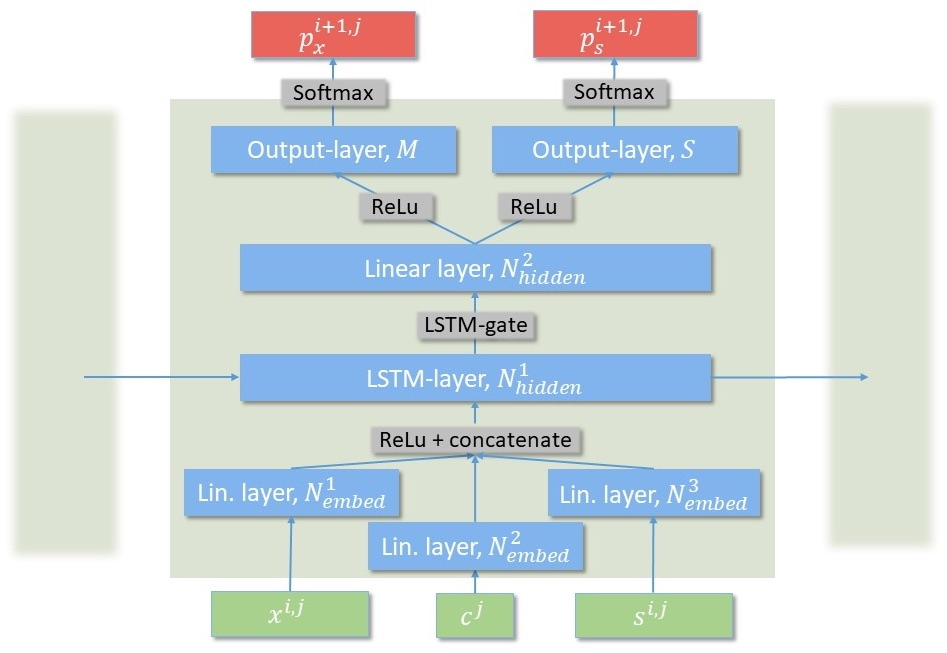
\includegraphics[width=0.7\textwidth]{images/LSTM_design_new2.jpg}
\caption{Architecture of the LSTM network for modelling sequences of network flows.}
\label{fig:LSTM}
\end{figure}

Since the paper is now in under my responsibility, and due to all the efforts I put into its improvement, we agreed that I would be the first author of this work in the event of publication. Unfortunately, due to the difficulties describes in Section \ref{Sec:Problems}, we were so far unable to get this work accepted at a suitable venue. We first submitted the manuscript to the ACSAC conference, where the general consensus was that the application of LSTM networks for network anomaly detection is not novel enough, and that there is not enough connection between the used methodology and the detected attacks.
After efforts to improve on these issues, we attempted a revised manuscript to the CODASPY conference. Again, the main criticism here was novelty and scope of the methodology, and scepticism about the translation of results to real-world application. After more thorough revisions, highlighting of the papers novelty as well as the addition of additional modern baseline models, we have submitted a new manuscript to the DIMVA 2020 conference as a final attempt. 

Due to these difficulties, I spent a lot more time with this project than I originally intended, in total about 6.5 months. We are awaiting the response of the reviewers at the DIMVA 2020 conference, but do not intend to further pursue any substantial flow-based models.



\subsection{Traffic Generation using Containerization for Machine Learning}

Building contextual models of network traffic means to build an understanding how different network interactions can be distinguished via their traffic trace. However, available network traffic datasets do not contain ground truth labels about the nature of computer interactions and often suffer from a lack of realism. To improve this and ensure that our models extract meaningful sets of sequences that represent these different interactions, we started developing a containerised traffic generation framework to generate traffic with ground truth labels. 

%Network traffic datasets are already hard to obtain due to privacy concerns. However, as  the correspondence between individual network traffic events and their particular purpose is virtually never recorded on a computer, very few datasets contain ground truth about the captured events. For that reason, a particular aspect of this project is to generate useful ground truth data with appropriate content myself.

This framework generates controlled and isolated network traffic from a variety of applications and tasks. For this, a virtual network was created using the virtualisation program \textit{Docker}. In this network, two or more parties can communicate through containers,  which are sandboxes containing programs inside a minimal virtualised operating system. The benefit of this design is that individual containers can only communicate with each other via the virtualised network while the host is in complete control of the parallel execution of tasks in multiple containers. To capture the traffic, every container in the network was complemented with a \textit{tcpdump}\footnote{A common packet capture utility} container hooked onto the network interface. The captured traffic can then be labelled according to the particular scenario it was generated by. We implemented a variety of network service  scenarios to capture a diverse set of network traffic.

\begin{figure}
\centering
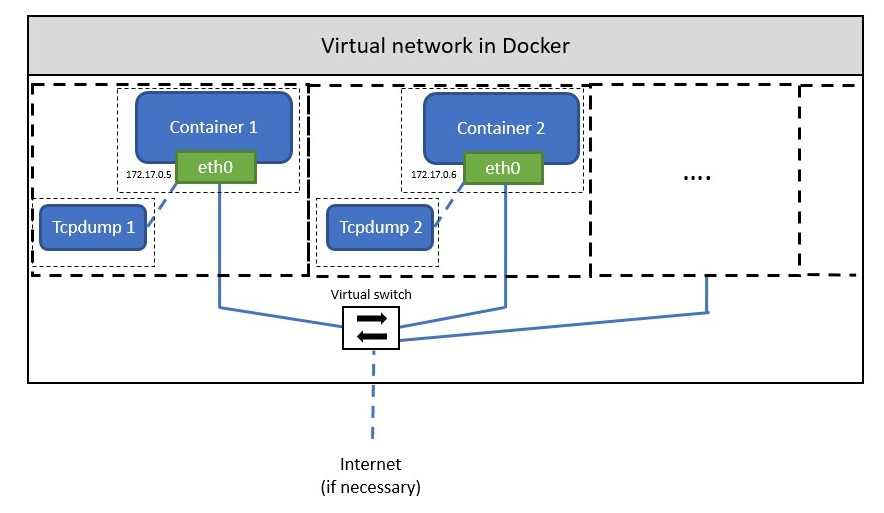
\includegraphics[width=0.7\textwidth]{images/Dockernet.jpg}
\caption{Visualisation of the virtual network in Docker}\label{docker}
\end{figure}


We emphasised the following particular strengths in our framework, which makes the generated data particularly suitable for ML-applications:
\begin{itemize}
\item traffic variation through a diversity of generation scenarios as well as transmission disturbances,
\item ground truth labels through containerised separation of generation scenarios,
\item scalability of the amount of generated traffic,
\item and modularity of the framework to easily extend and update the set of scenarios.
\end{itemize}



This work was started in summer 2018 by me and Nikola Pavlov\footnote{an LFCS summer intern}, and continued in summer 2019 by me and Robert Flood\footnote{an LFCS MSc student}. My responsibilities lied in overall design of the framework as well as the requirements on the generation features, testing and extending individual scenarios as well as implemention, and the design and conduction of validation experiments. 

In autumn of 2019, Robert Flood and I described the framework in a paper of which I am first author, which was submitted and accepted at the ACSAC DYNAMICS workshop 2019, and will appear in the corresponding proceedings this March. 

Due to very positive feedback at the workshop as well as encouragements and suggestions to extend the framework, we are working further on this project, which is described in Section \ref{Sec:dockerext}.

\subsection{Stint at BT - Stepping stone detection and connection correlation}\label{Sec:BTstint}

As part of my CASE PhD scholarship, I spent six weeks with my industrial sponsor at BT Labs Adastral Park in August and September 2019. Before starting this stint, I met with my industrial supervisors to define a project to work on that is both related to my PhD and is a relevant problem for BT. During this meeting, we agreed that the problem of detecting stepping stones was a suitable topic. 

In a stepping stone scenario, an attacker launches an attack not from their own computer but from intermediary hosts within an enterprise network that were previously compromised, often using an interactive relay session. A common approach in the literature to detect stepping stones is to identify correlation between an two connections on a potential intermediary host. Attackers try to evade detection by inserting chaff packets and delays to make the connection appear uncorrelated.

The biggest challenge for this problem is that there are no available datasets available that describe stepping stone behaviour. Due to the success of the implemented traffic generation framework, I started to implement several scenarios of interactive traffic relays using ssh-tunnels and netcat/netem for chaff and delay insertion. With this, I was able to generate significant amounts of traffic with a controllable amount of noise and delay to train and assess correlation models. 
I furthermore implemented a state-of-the-art method for connection correlation \cite{nasr2018deepcorr} that uses a deep convolutional neural network as a benchmark to compare a future model with. 


\begin{figure}
\centering
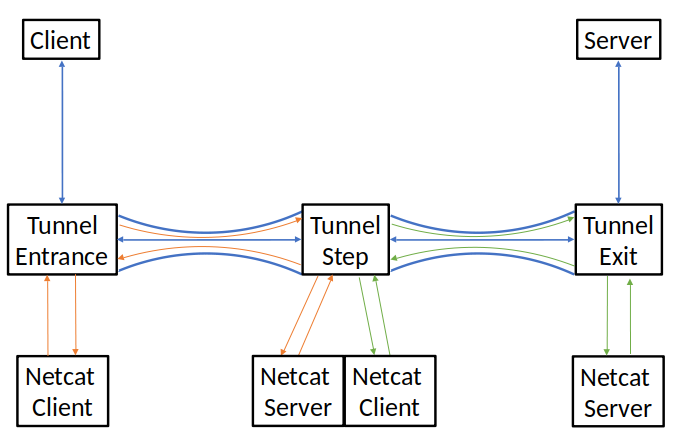
\includegraphics[width=0.7\textwidth]{images/Step_stones.png}
\caption{Implementation of ...}\label{stepstone}
\end{figure}

After finishing the stint at BT Labs, I continued to work on the traffic generation for a bit further before we had a call with Jake Hill, a security expert at BT. This call was meant to provide field knowledge to confirm and/or improve the data generation set-up. However, Jake stated that the problem of attackers launching attacks from intermediary hosts is after all not of great relevance for BT's operations. Instead, his notion of stepping stones described simple proxies relaying services (more on this in Section \ref{Sec:Relay}). In addition, further investigation suggests that the consensus in the literature is that connection correlation produces too many false positives and is not applicable in real-world scenarios. 

\subsubsection{Scope of the project for publication}

With this information, I decided to scale this project down and produce a simple evaluation of existing connection correlation methods. Since the major contribution of this work so far is the large amount of detailed and varied data I can produce, this allows for the first time an independent assessment of existing methods. So far I have implemented and evaluated four different methods, and am in the process of finishing this project. I am currently producing a small paper from it, which I intend to publish at a smaller workshop or conference. 






\subsection{Modelling of connection establishment via LSTM encoders}\label{Sec:Encoder}

The distinct contextual behaviour of an applications manifests itself most clearly in the first few packets exchanged in a connection. This is the stage in a connection during which a specific client or server request is transmitted, encryption keys are exchanged, users authenticate themselves with passwords, ports for successive connections are defined, etc. This distinction goes far beyond individual traffic protocols, as even a single application usually can exert different actions which translate to different contextual behaviours in this initial negotiation phase. 

The significance of the initial negitiation phase is bolstered by two publications on the area of traffic classification that share the same conclusion and train clusters and classifiers on the metadata of the first five to ten packets to distinguish different applications \cite{bernaille2006traffic,crotti2007traffic}.

Learning precise contextual representations of this initial negotiation phase from applications running on a computer has several main benefits for this project: 

\begin{itemize}
\item Several types of attacks exploit loopholes accessible at the negotiation stage. A precise contextual representation model could detect anomalous deviations in particular packet parameters from the learned behaviour. A simple example of such a deviation from expected behaviour would occur during a \textit{buffer overflow attack}, which overflows an input buffer (such as for a password) to directly modify memory locations. This should be observable as a significant deviation in the corresponding packet size.

\item Newly installed malware will most likely exhibit different than normal behaviour in this stage, from very different negotiation procedures to just slight deviations in the packet interarrivals.

%\item The translation of contextual negotiation structures into different behaviour groups could be used to associate the corresponding flow with particular actions, i.e. to give the flow one or more labels. To be meaningful, the identified groups have to correspond to actual contextual behaviours and should be consistent along similar actions. 
%Such a flow labelling could be very helpful for understanding contextual structures of flow traffic, and consequently for anomaly detection on a higher level, such as the described work by Chen et al.\cite{chen_more_2016}. I will describe this more in Section \ref{Curmet}.

\item Malicious traffic that tries to disguise itself by using common ports can be identified as a \textcolor{red}{behavioural mismatch}.

%\item As applications are updated, their particular traffic generation distribution $P(X)$ can also  gradually change, causing corresponding traffic to be potentially flagged as anomalous by current anomaly detection methods. A representational model could identify common contextual substructures between traffic instances and thus indicate that they originate from an updated application. More detail will be given in Section \ref{Robustness}.

\end{itemize}

In order to generate accurate representations of negotiation phases, I have implemented an LSTM-autoencoder model that can simultaneously work as an anomaly detection model as well as an embedding generator for sequence clustering. I have tested this model on initial test-datasets, on which it achieves excellent results while being able to spot anomalies accurately. I have also added a simple k-nearest neighbour clustering algorithm, however its performance will have to be evaluated on a larger dataset. 

\begin{figure}\label{LSTM_Enc}
\centering
\begin{subfigure}[b]{0.5\textwidth}\label{LSTM1}
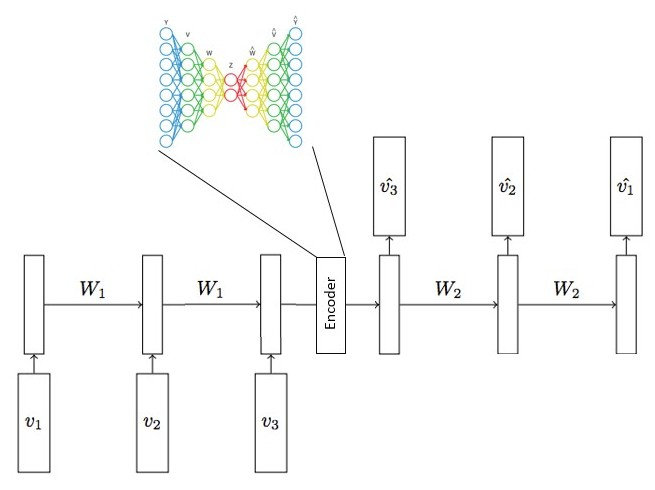
\includegraphics[width=\textwidth]{images/LSTM_Encoder.jpg}
\caption{}
\end{subfigure}
\begin{subfigure}[b]{0.34\textwidth}
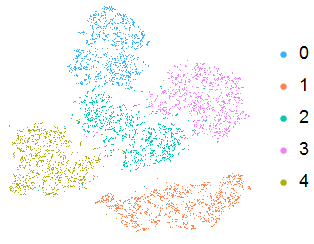
\includegraphics[width=\textwidth]{images/MNIST.png}
\caption{}\label{LSTM2}
\end{subfigure}
\caption{Visualisation of the design of an LSTM Autoencoder (a), taken from https://machinelearningmastery.com/lstm-autoencoders/, and the embedding of different types of handwritten digits by an autoencoder.}
\end{figure}

\subsection{Scope of the project for publication}

Due to the difficulties described in Section \ref{Sec:Problems} of publishing anomaly-based methods in network intrusion detection, we are currently rethinking the scope this project should take for publication. One idea is to pitch it simply as a traffic classification and clustering method, since the evaluation and applicability demonstration is more straightforward.


\section{Future plans}

\subsection{Submission of Stepping stone project and negotiation phase model}
%\section{Introduction and motivation}

With work being almost finished for the stepping stone project and the negotiation phase model also being well on the way, I am planning to write each project up into a paper for publication. Since the scope for each project was scaled back a bit, I am intending to submit them to smaller venues with a higher acceptance rate, and do not intend to spent more than three months completing both. \textcolor{red}{find venue}.

\subsection{QUIC anomaly detection}

An advice I received at the ACSAC conference from Guofei Gu, the Program Chair, was to identify very specific and novel applications of machine learning methods to intrusion detection in order to produce publications that could be accepted at renowned venues. One such applications could be to the new transport layer QUIC. QUIC seeks to improve performance of connection-oriented web-applications using TCP. It is implemented on top of UDP and implements its own TCP-like packet control mechanisms. It allows for multiplexed HTTP-connections and resolves head-of-line blocking during packet loss as well as reducing latency by minimising round-trips during connection establishment. Furthermore, much of the QUIC implementation is moved from kernel to user space, which allows continuous updates of the protocol.

According to an NGINX-spokesperson, "since the protocol is new and things like stack optimization etc. still to catch up and since it's all user-space, there is a possibility to make changes to protocol very rapidly. This generates a higher attack surface than you would have over more layered approach with TCP and http on top." Initial investigations showed that there exists no research on mitigating intrusions over the QUIC protocol.%, which \textcolor{red}{...}


\textcolor{red}{Due to the implementation in user-space}, QUIC may introduce vulnerabilities that allow remote code execution on a host, such as in \textit{CVE-2017-15407} and \textit{CVE-2017-15398}. The detection of such code executions by building a combined model of QUIC packet exchanges and process starts/system calls therefore seems like a promising project that provides both novelty and relevance.

In particular, I believe the following conditions would allow for interesting results:
\begin{itemize}
\item Operation on a host (server or client) level
\item Combination of unencrypted packet packet stream and system calls/process starts corresponding
\item A sequential model that applies NLP-techniques to packet content and predicts probability of process start or particular system call (which could then correspond to code execution)
\item Traffic and system call/process log collection using a containerized framework.
\end{itemize}

One difficulty in this project is that there do not exist many identified vulnerabilities in the QUIC protocol yet, of which none are known to have been used in a successful attack. Therefore, it might be difficult to get enough malicious data for result validation. In total, I would asign four months work in this project to conclude.




\subsection{Service relay detection}\label{Sec:Relay}

As mentioned in Section \ref{Sec:BTstint}, disussion with a security expert at BT Labs indicated that the detection of simple proxy servers that relay protected services to third parties from the perspective of an ISP is a relevant and promising research project. Specific characteristics of this problem are:

\begin{itemize}
\item Unlike the original stepping stone problem, these relay proxies operate in a simplistic fashion and do not use evasion tactics. However, content can be forwarded using a different application or protocol than in the first connection.
\item Packets are sampled before observation, meaning that only every n-th packet for each connection is observed.
\item Benign proxies exist that can increase false-positives.
\end{itemize}

Initial investigations that I conducted showed that there are no publications yet that address this problem in any way, which indicates the potential for novel contributions. Since there exists no description or analysis of such proxies at all, this however also means that we are reliant on BT for knowledge and guidance on the problem definition and proxy operation mode. Also since no public dataset exists, we would have to implement and generate our own dataset and feedback with BT to check if it resembles the behaviour of such proxies, . At the moment it seems that a suitable start would be to focus on video relay. Necessary steps for this project are:

\begin{itemize}

\item Implement a docker traffic generation scenario to generate realistic data, and parse them in a sampled manner.
\item start designing and implementing detection methods. As there are no evasion tactics involved, simple cumulative sum or moving window statistics with a p-value threshold seem like a good start.
\item Test these methods on the data with a suitable background of independent connections as well as benign proxies. Obtaining simple background data is not challenging, however we will have to discuss how and to what extend benign proxies should be included in the background data.
\item Evaluate and adjust/improve existing methods.

\end{itemize}

As we are reliant on the cooperation with BT Labs, we are not completely certain yet if this project will go ahead yet. We will have a further discussion with them later this month, which will bring more clarity. 

\subsection{Extension of Docker framework}\label{Sec:dockerext}

Due to very positive feedback at the workshop as well as encouragements and suggestions to extend the framework, Robert Flood and I are working further to extend the current traffic generation framework. Particular goals are:

\begin{enumerate}
\item Extend the framework to create datasets that resemble full fledged computer network with variable topology. For this, several subtasks need to be completed:

\begin{enumerate}

\item Embed all scenarios in a \textit{Mininet} framework in order to allow the fast inclusion of switches, routers, etc.

\item Build a mechanism that can generate variable or random network topologies.

\item Create a launch mechanism that starts and executes different traffic scenarios for a given network topology at times and locations drawn from appropriate distributions that resemble empirical network behaviour.

\end{enumerate}
\item Include the collection of application logs and system call logs for each container. These will then be matched with the corresponding traffic captures and receive the same ground truth labels.

\item Generate different multi-step attack executions on a set of network topologies to capture the similarities and disimilarities between different attack techniques and tactics.

\end{enumerate}

Since I am not the lead on this project, I currently do not have a timescale for its completion.


\subsection{Thesis submission}

In the light of the problems described in Section \ref{Sec:Problems} that we encountered in the field of anomaly-based intrusion detection, I believe that the \textcolor{red}{theme} of this PhD-project has to be altered \textcolor{red}{a bit}. 

reoccurring theme traffic generation for specific machine learning applications, and ML applications as examples

All applications so far driven by traffic generation:
\begin{itemize}
\item stepping stone
\item traffic relay
\item LSTM encoder
\item QUIC anomaly detection?
\end{itemize}



%\addcontentsline{toc}{section}{Bibliography}
\bibliographystyle{abbrv}
\bibliography{refs}

\end{document}